\label{standard-call}
\subsubsection{Purpose}

Any subscribed passenger shall be able to request a taxi either through the web application or the mobile app.
After the request, the passenger is informed by the system about the waiting time and the code of the incoming taxi.

Requests shall be forwarded to available and active taxi drivers in the same zone of the passengers. Taxi drivers shall be able to accept or reject an incoming request.

\subsubsection{Scenario 1}
Alice needs a taxi. She opens the myTaxiService mobile app on her phone, and selects ``Call a taxi''. She authorizes the application to access her GPS data, checks on the map that her position is correct and confirms the request.

The system forwards the request to Bob, the first taxi driver in Alice's taxi zone. Bob decides to accept the call: a map of Alice's position gets displayed on Bob's phone and the navigator starts.

Bob's position is transmitted from his phone to the system, which computes the ETA for the incoming taxi and shows it to Alice. Bob arrives and picks Alice up. Then he confirms that the passenger is on board.

When the ride is over, Bob taps on ``Finish ride'' so that the system knows that Bob is ready for another ride.

\subsubsection{Scenario 2}
Luke needs a taxi. He requests it and the request is forwarded to the first taxi driver in queue, Chewbacca. Chewbacca decides to reject the incoming request, so the system puts him at the bottom of the queue.

Luke's request gets forwarded to the new first taxi driver in queue, Han Solo. Han accepts the request and comes to pick up Luke.

\subsubsection{Scenario 3}
Luke, Leila and Obi-Wan need a taxi. Luke has myTaxiService app on his phone so he opens it and selects ``Call a taxi''. He checks that position is correct, he enters three as number of seats required and confirms the request.

Luke's request gets forwarded to the first taxi driver in queue, Han Solo, that accepts the request and comes to pick up the group of friends.


\begin{figure}
\begin{center}
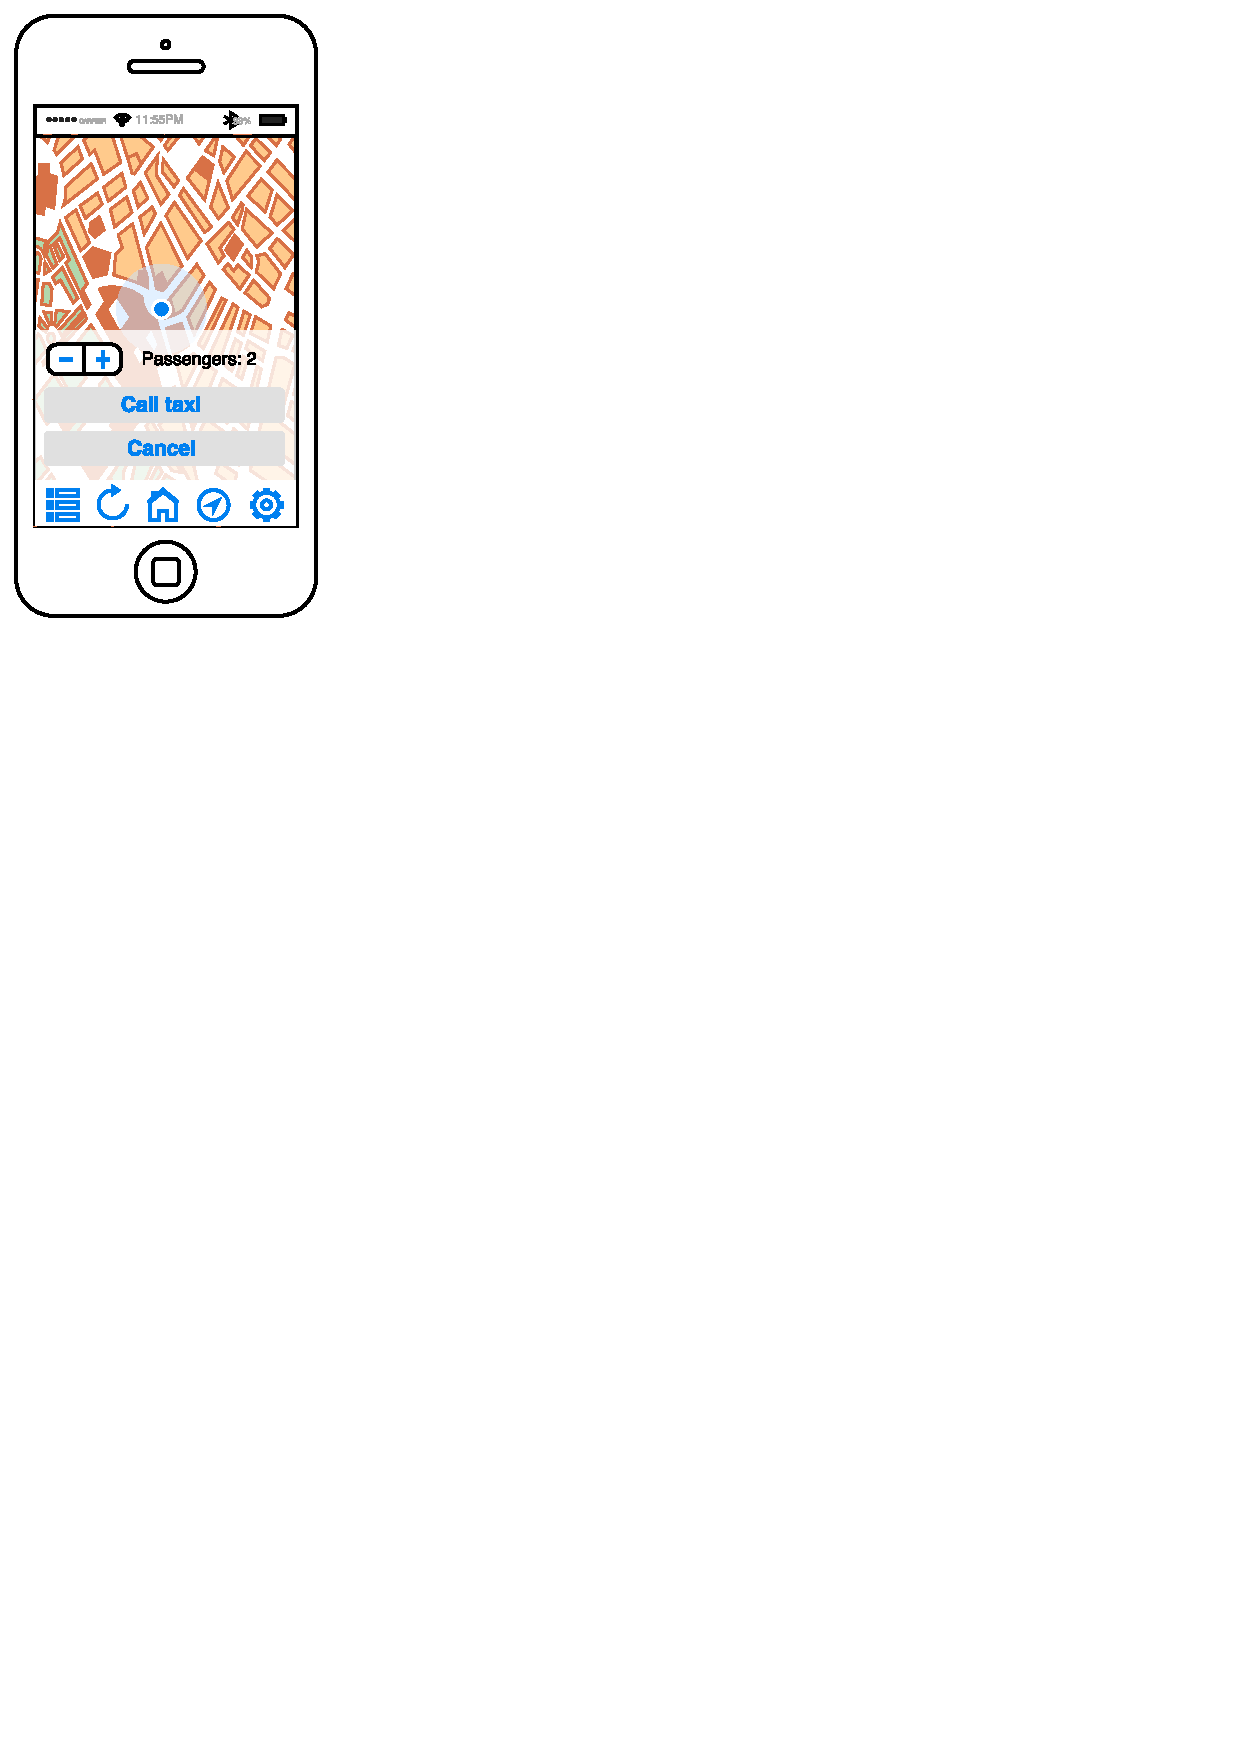
\includegraphics[width=0.4\textwidth]{mockup/TaxiCall.pdf}
\caption{Concept of the taxi call interface.}
\label{fig:mockup-taxicall}
\end{center}
\end{figure}

\subsubsection{Use case}
The use case for a taxi call is shown in~\autoref{usecase-taxicall}.

\begin{table}
\begin{center}
\begin{tabular}{| l | p{0.6\textwidth} |}
\hline
Actor & Passenger \\
\hline
Goal & Goal~\ref{g-taxicall}
\\
\hline
Input condition & Passenger is already logged in and requests a taxi.  \\
\hline
Event Flow & \begin{enumerate}
	\item The passenger requests a taxi through the client.
	\item The request gets forwarded to the first taxi in the queue of the same taxi zone of the user.
	\item The taxi driver can either accept or deny the request; if he denies it, the request is forwarded to the next taxi driver in the queue, and so on.
	\item Finally the request gets accepted by a taxi driver.
	\item The passenger gets notified that a taxi driver accepted his request and is given the ETA of the incoming taxi.
	\item When the taxi driver meets the passenger, he/she signals that the passenger is on board.
\end{enumerate}
\\
\hline
Output condition & The driver confirms that the passenger is aboard. \\
\hline
Exception & No taxi is available in the passenger's zone. \\
\hline
\end{tabular}
\end{center}
\caption{Use case for a standard taxi call.}
\label{usecase-taxicall}
\end{table}

\subsubsection{Response sequence}
The response sequence is illustrated in figures \ref{fig:sequence-taxicall} and \ref{fig:sequence-taxicall-refused}.

\begin{figure}
	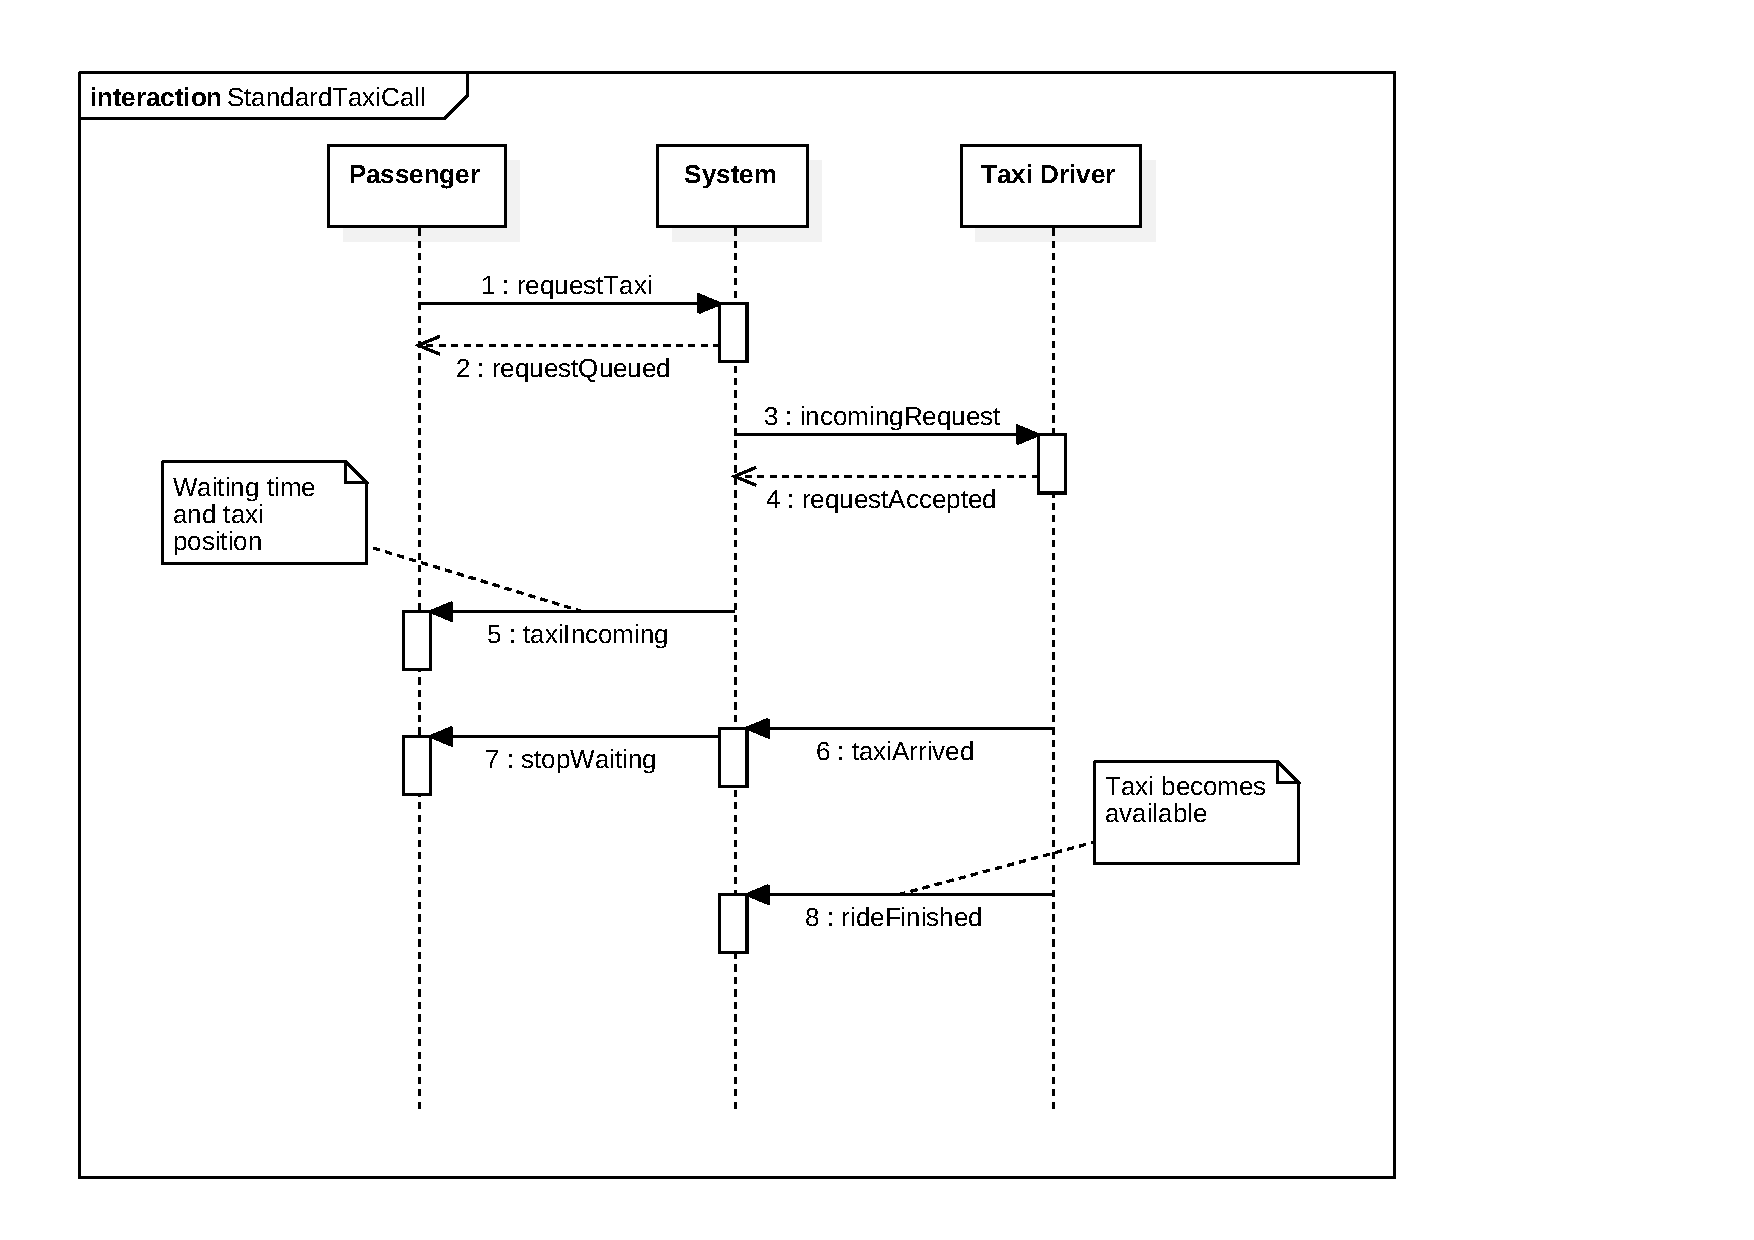
\includegraphics[width=\textwidth]{diagrams/sequence_taxicall.pdf}
	\caption{Sequence diagram of a successful taxi call, picked up by the first taxi driver called by the system.}
	\label{fig:sequence-taxicall}
\end{figure}

\begin{figure}
	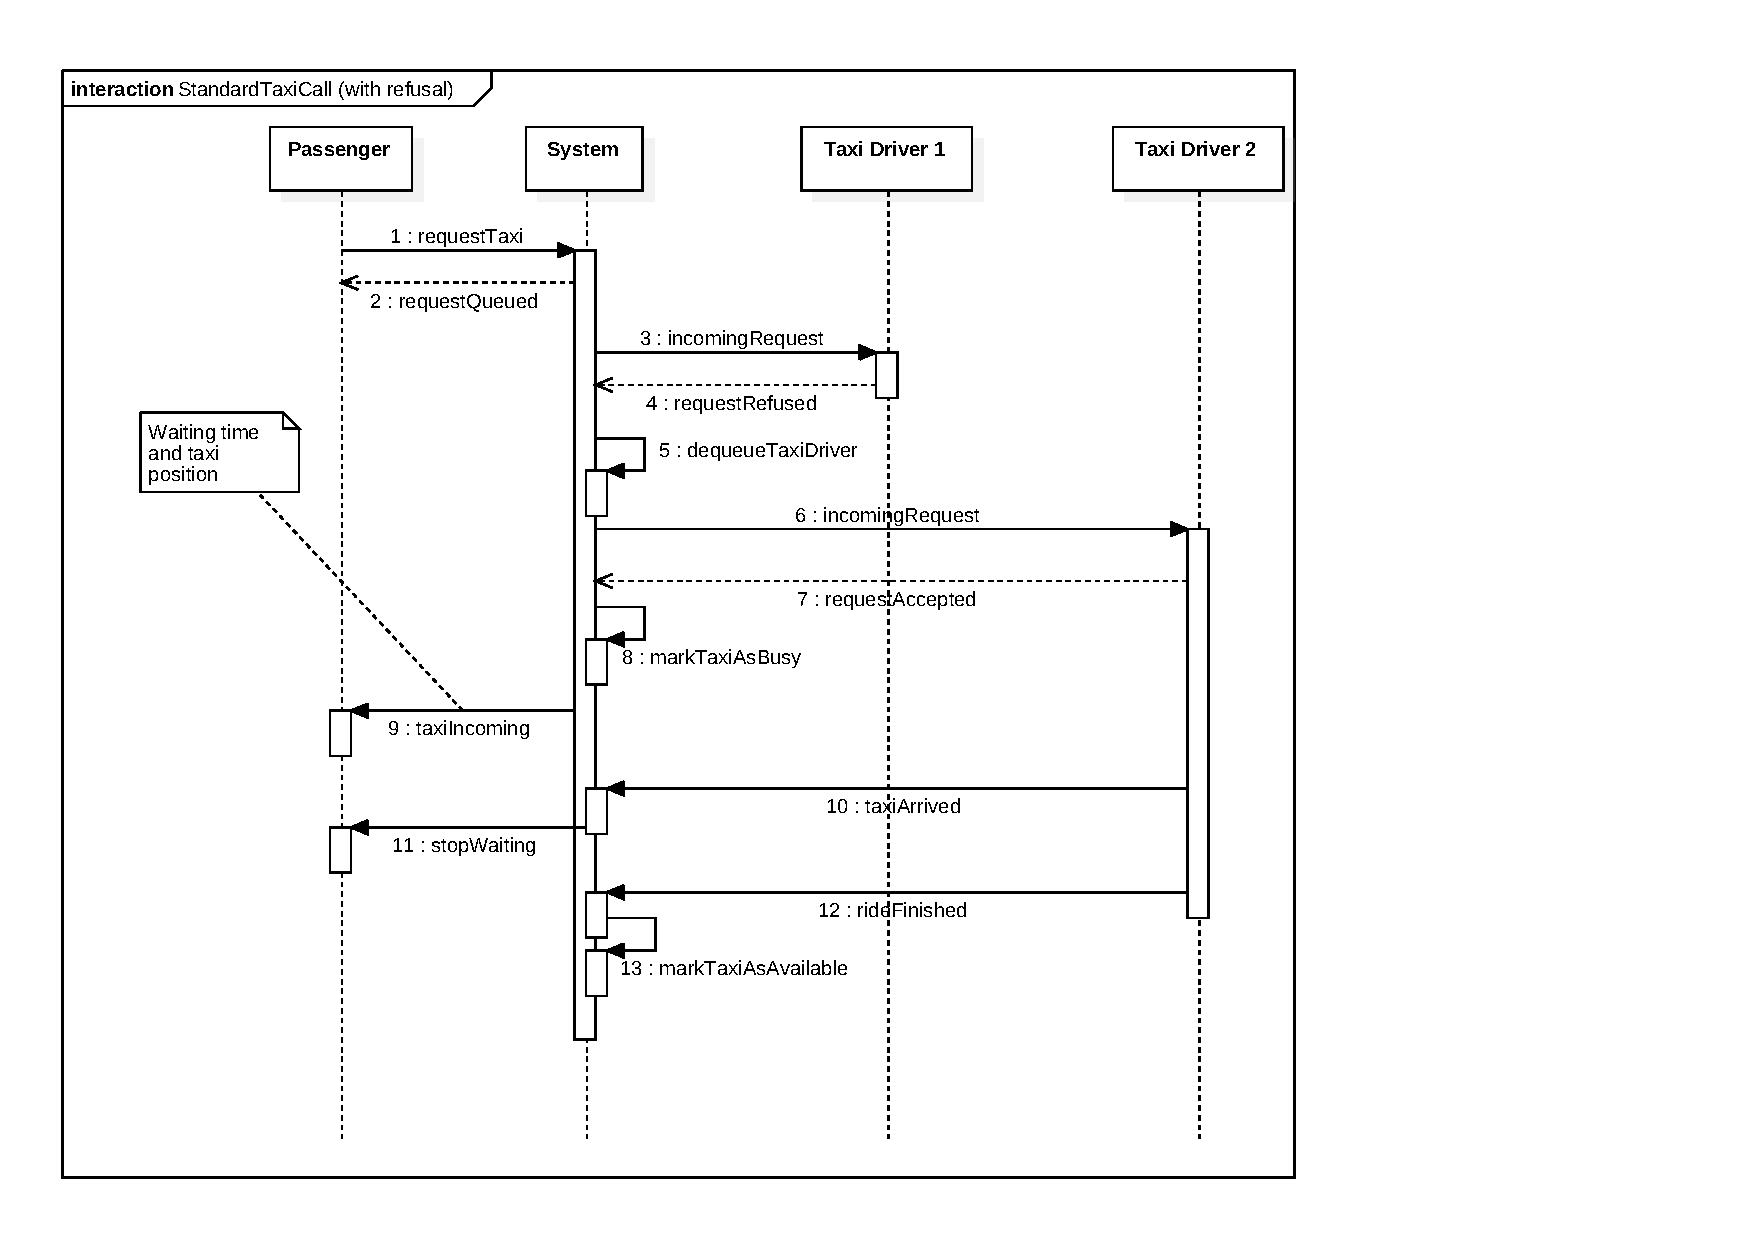
\includegraphics[width=\textwidth]{diagrams/sequence_taxicall_refused.pdf}
	\caption{Sequence diagram of a taxi call when the first taxi driver to receive the request refuses the call and the second one accepts it.}
	\label{fig:sequence-taxicall-refused}
\end{figure}

\subsubsection{Associated functional requirements}
\begin{enumerate}
	\item The system must localize the passenger before he or she makes a taxi request.
	\begin{enumerate}
		\item (App) If GPS info is available and the passenger can be tracked within a radius of 50 m, then the passenger is presented with the option of using the current GPS position.
		\item (App) If GPS info is not available or the precision is less than 50 m, then the app requests the passenger to insert a valid address. Then the address is shown on a map and the passenger can confirm its position.
		\item (Web) In the web application the user is always requested to insert a valid address. Then the address is shown on a map and the user can confirm its position.
	\end{enumerate}

	\item When the system knows the passenger's position, it asks the number of seats required in the taxi.
	\item Once the system knows the number of seats required, it presents the passenger the option to request a taxi.
	\item The system must ask the passenger for confirmation before delivering the taxi request.
	\item After the passenger's confirmation of a taxi request, the request is delivered to the first taxi with a sufficient number of seats in the queue for the taxi zone in which the user is located.
	\item Taxi requests are forwarded only to active taxi drivers which are located in the same taxi zone, who are not currently busy.
	\item Taxi requests are processed in order of arrival.
	\item If there's no taxi driver in the passenger's taxi zone, the request is refused and en error message is displayed to the passenger.
	\item When a taxi driver receives a request, the mobile application shows a notification and emits a sound.
	\item When receiving a request, the taxi driver is presented with the possibility of accepting or denying it.
	\item After having accepted a request, the taxi driver is automatically marked as ``busy''.
	\item After having accepted a request, the mobile application shows to the taxi driver a map with the location of the passenger, and automatically starts navigation instructions on the app preferred by the taxi driver (Google Maps, Waze, TomTom, etc.).
	\item After the taxi request is accepted, the app shows the passenger a map with the current position of the incoming taxi.
	\item After the taxi request is accepted, the passenger is informed about the ETA for the incoming taxi.
	\item The ETA for the incoming taxi is fetched from the server every 90 s.
	\item The ETA for the incoming taxi is computed by the system considering the distance from the taxi to the passenger and the current traffic conditions.
	\item When the taxi is within 20 m from the passenger, the app asks the taxi driver to confirm that the passenger is aboard.
	\item When the taxi driver confirms that the passenger is aboard, the taxi request is marked as fulfilled and the system stops showing the waiting time to the passenger.
	\item The system must prevent the passenger to call a taxi while he/she is already waiting for one.
	\item The system must prevent the passenger to call a taxi while he/she is already travelling in a taxi.
\end{enumerate}
